\section{OST and obdfilter}
\label{sec:ost-and-obdfilter}

\begin{quote}
\begin{Verbatim}
/* Sigh - really, this is an OSS, the _server_, not the _target_ */
static int ost_setup(struct obd_device *obd, obd_count len, void *buf)
{ ... }
\end{Verbatim}
\begin{flushright}
\textit{\small from Lustre source tree b16}
\end{flushright}
\end{quote}

Lustre source tree \url{lustre/ost} and all function names prefixed with
\url{ost_} should probably be regarded as server (OSS) functions, if we
understand the above comment correctly.

\subsection{OSS as OST}

OST is loaded as a kernel module. It works closely with obdfilter and does most
of the server/OST side of the work. Between these two layers, OSS is the switch
layer or the \textit{thin} layer, and it interprets requests from Portal RPC,
prepares for requests, and then passes requests to obdfilter for further
processing. In the following discussion, we focus on two aspects of it: initial
setup and switching structure, implemented by \url{ost_setup()} and
\url{ost_handle()}, respectively.

\subsubsection*{Initial Setup}

\begin{itemize}

\item First, the OST checks if the OSS thread number is specified. If not, then it
computes the minimum number of threads based upon the CPU and memory and
ensures that there is 4x dynamic range between the minimum and maximum number
of threads. 
\begin{Verbatim}
    oss_min_threads = num_possible_cpus() * num_physpages >> (27 - CFS_PAGE_SHIFT);
    if (oss_min_threads < OSS_THREADS_MIN)
         oss_min_threads = OSS_THREADS_MIN;
    /* Insure a 4x range for dynamic threads */
    if (oss_min_threads > OSS_THREADS_MAX / 4)
         oss_min_threads = OSS_THREADS_MAX / 4;
    oss_max_threads = min(OSS_THREADS_MAX, oss_min_threads * 4 + 1);
\end{Verbatim}


To get the obd device of the OST; the following function call is used.

\begin{Verbatim}
struct ost_obd *ost = &obd->u.ost;
\end{Verbatim}

\item Then, the server side initiates RPC services by:
\begin{Verbatim}
ost->ost_service = ptlrpc_init_svc( , , , , , , ost_handle, , , , "ll_ost");
\end{Verbatim}

The function returns the pointer to struct \url{ptlrpc_service}. One important
thing to note is that we have supplied a handler, \url{ost_handle}.  Once the
service is set up as shown below, Portal RPC will dispatch the request to this
handler for further processing. That is the subject of the following
section.

\item The prtrpc threads are started as:

\begin{Verbatim}
rc = ptlrpc_start_threads(obd, ost->ost_service);
\end{Verbatim}

\item The similar call sequence is repeated for creating \textit{ost create}
threads and the returned service handle is assigned to
\url{ost->ost_create_service}. It is also repeated for \textit{ost io} threads,
and a service handle is assigned to \url{ost->ost_io_service}.

\item And finally, the ping eviction service is started.

\end{itemize}

\subsubsection*{Dispatching}

The handler function takes one input parameter, \url{struct ptlrpc_request
*req}, and it is driven largely by the type of request.  The decoding of type of
request is through passing \url{req->rq_reqmsg} (which points to struct
\url{lustre_msg}) to a helper function \url{lustre_msg_get_opc()} provided by
Portal RPC. Thus the dispatch structure looks like:

\begin{Verbatim}
swtich (lsutre_msg_get_opc(req->rq_reqmsg)) {
case OST_CONNECT: 
    ...
    rc = target_handle_connect(req, ost_handle);
    break;
case OST_CREATE:
    ...
    rc = ost_create(req->rq_export, req, oti);
    break;
case OST_WRITE:
    ...
    rc = ost_brw_write(req, oti);
    RETURN (rc);
case OST_READ:
    ...
    rc = ost_brw_read(req, oti);
    RETURN(rc);
}
\end{Verbatim}

The exception handling includes the possible recovery, which can happen during
any request except the \url{OST_CONNECT}. Also, we need to check for connection
coming from an unknown client by checking \url{NULL} of \url{req->rq_export}.


\subsection{OST Directory Layout}

This section describes what you will observe on the disk when logging onto an OST
node. The filesystem on the disk is most likely \textbf{ldiskfs} for now. It
means the backend data is really stored as a regular file, organized in a
certain Lustre specific way:

\subsubsection*{Group Number}

Under the top level directory on an OST is the subdirectory named for each group. 
This layout accommodates clustered MDSs where each group corresponds to
one MDS. As of now, only one MDS is in use, so only group zero is effective.
\footnote{In fact, there is a special group for echo client as well, so that
MDS and echo client do not conflict when run at the same time.}

\begin{comment}
\subsubsection*{Stripe Number} 

Data objects of a file are numbered from zero.  Inside Lustre, you will see
\url{int stripeno} that denotes the particular index of the data object
\textit{within} the file.
\end{comment}

\subsubsection*{Object Id}

Under each group, 32 subdirectories are created. For each file object, its
last five digits are used to identify which subdirectory this file should reside
with. Here, the filename is the object id.

\subsection{obdfilter}

The obdfilter device is created when the OST server is initialized. For each
OST, we have an associated obdfilter device. For each client connection, the
obdfilter creates an export as the conduit of communication. All the exports
are maintained in a global hash table, and the hash key is also known as UUID,
as shown in both Figure \ref{fig:obdfilter_conns} and \ref{fig:exp}. The
Portal RPC layer makes use of UUIDs to quickly identify to which export (and
obdfilter device) the incoming request should go. Also, each obdfilter device
maintains a list of the exports it is serving. This relationship is
illustrated in Figure~\ref{fig:obdfilter_conns}. 

\begin{figure}[htb]
\centering
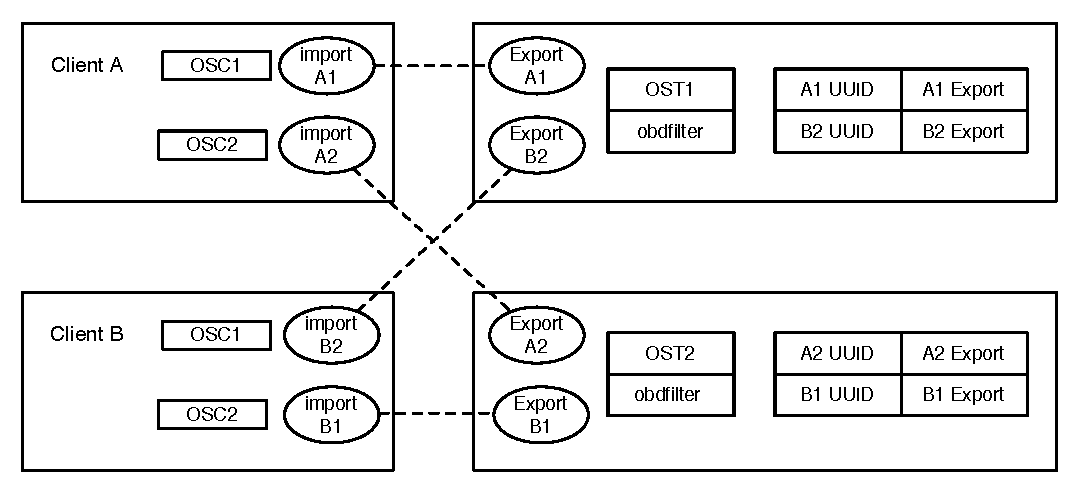
\includegraphics[width=4.5in]{img/obdfilter_conns}
\caption{Import and export connections between an OSC and obdfilter.}
\label{fig:obdfilter_conns}
\end{figure}

The obdfilter provides the following functions:

\begin{itemize}
  
  \item handles create request, presumably from MDS for file data
  objects.

  \item handles read and write requests, from OSC clients.

  \item handles connect and disconnect requests from lower Portal RPC layer for
  established exports and imports.

  \item handles destroy (which involves both client and MDS) requests.

\end{itemize}

\subsubsection{File Deletion}

The destroy protocol is as follows. First, the client decides to remove a file and
this request is sent to MDS. MDS checks the EA striping and uses \url{llog}
to make a transaction log. This log contains the following:
$<$\textit{unlink object 1 from ost1, unlink object 2 from ost2, etc.}$>$.
Then, MDS sends this layout and transaction log back to the client. The
client takes this log and contacts each OST (actually obdfilter) to unlink each
file object. Each successful removal is accompanied by a confirmation or
acknowledgment to the unlink \url{llog} record. Once all unlink llog records on
MDS have been acknowledged, the file removal process is completed.


\subsubsection{File Creation}

As discussed earlier in Section \ref{sec:ost-and-obdfilter}, all requests are
handled by OST and obdfilter together.  Now, we will walk through the handling
of a create request. The first portion of request handling is done inside
\url{ost_create()} as follows.

\begin{enumerate}

\item Prepare the size of reply message. It is composed of two records and thus
requires two buffers. The first record is for portal rpc body, and the second,
for the ost reply body.

\begin{Verbatim}
__u32 size[2] = { sizeof(struct ptlrpc_body), sizeof(*repbody)};
\end{Verbatim}

\item Get a pointer to the request body from the original request and do
byte swapping when necessary.

\begin{Verbatim}
struct ost_body *body = lustre_swab_reqbuf(req, REQ_REC_OFF,
            sizeof(*body), lustre_swab_ost_body);
\end{Verbatim}

The last parameter is the swab handler, which is called only when the swapping is
necessary. Client side uses native byte order for its request, along with a
pre-agreed magic number. Server side reads the magic number to decide if a swap
is needed.

\item Do the actual space allocation, and fill in preliminary header
information.

\begin{Verbatim}
rc = lustre_pack_replay(req, 2, size, NULL);
repbody = lustre_msg_buf(req->rq_repmsg, REPLY_REC_OFF,sizeof(*repbody));
\end{Verbatim}

After the first call, \url{req->rq_repmsg} points to the newly allocated
space. The second call assigns \url{repbody} of the starting address for the buffer
of the reply body.

\item Finally, it fills in the reply body with exactly the same contents as a
request body and passes on to obdfilter for further processing.

\begin{Verbatim}
memcpy(&repbody->oa, &body->oa, sizeof(body->oa));
req-rq_status = obd_create(exp, &repbody->oa, NULL, oti);
\end{Verbatim}

\end{enumerate}

For the create request, the entry point for obdfilter is through
\url{filter_create()}. 

\begin{Verbatim}
static int filter_create(struct obd_export *exp, struct obdo *oa ..)
\end{Verbatim}

We ignore the processing related to \url{struct lov_stripe_md **ea} and
\url{struct obd_trans_info *oti} because the former is a legacy code and
is unlikely to be used in the future.

\begin{enumerate}

\item First, save the current context and assign this client its own operation
context. This is for specifying necessary information for the thread if it
wants to access the backend filesystem. It is like a sandbox limiting the
reach of server threads when processing requests from clients; it stores
``filesystem root'' and ``current working dir'' for the server thread (not
obtained from the client, of course, but rather dependent on which OST
we are working on).


\begin{Verbatim}
obd = exp->exp_obd;
put_ctxt(&saved, &obd->obd_lvfs_ctxt, NULL);
\end{Verbatim}

\item If the request is for recreating an object, then we cancel all extent
locks on the recreated object by acquiring the lock on the object and call on
\url{filter_recreate()} to do the actual job. Otherwise, we follow the normal
flow of precreating objects.  The reason for precreating is that, conceptually,
when MDS asks an OST for creating an object, OST doesn't just create one
object, it creates multiple objects with object id assigned. These batch
created objects have a disk size of zero.  The goal is, when MDS responds to a
client request next time for creating new file, it doesn't have to send a
request to OST again to present the layout information to client. By taking a
look at the pool of precreated objects from each OST, MDS may already have
all the information needed to reply to the client. 

\begin{Verbatim}
if (oa->o_valid & OBD_MD_FLFLAGS) && 
        (oa->o_flags & OBD_FL_RECREATE_OBJS)) {
    rc = ldlm_cli_enqueue_local(obd->obd_namespace, &res_id, ... );
    rc = filter_recreate(obd, oa);
    ldlm_lock_deref(&lockh, LCK_PW);
} else {
    rc = filter_handle_precreate(exp, oa, oa->o_gr, oti);
}
\end{Verbatim}

Here, \url{rc} returned from precreate handler is either a negative, indicative
of an error, or a non-negative number, representing the number of files created.

\item Now, we take a closer look at the function of precreate: 

When a client contacts an OST with a precreated object id, OST knows that this
object id now is activated. However, this presents a problem such that, if the MDS
has failed, it now has stale information on precreated
objects. To resolve this conflict, when MDS is restarted, it checks its records
on unused precreated objects and sends requests to OSTs to delete these
objects (\textit{delete orphans}). The obdfilter takes these requests and
skips those objects that are actually in use (but out of synchronization with
MDS's own record) and removes the rest of it. This is the first part of what
\url{filter_handle_precreate()} will do:

\begin{Verbatim}
if ((oa->o_valid & OBD_MD_FLFLAGS) && 
    (oa->o_flags & OBD_FL_DELORPHAN)) {
    down(&filter->fo_create_lock);
    rc = filter_destroy_precreated(exp,oa,filter);
    ...
} else {
    rc = filter_precreate(obd, oa, group, &diff);
    ...
}
\end{Verbatim}

\item Finally, the create request is passed onto \url{fsfilt} and is completed by
a VFS call. The process will later go through more steps, such as getting hold
of parent inode, transaction setup, etc.

\begin{Verbatim}
rc = ll_vfs_create(dparent->d_inode, dchild, 
                      S_IFREG | S_ISUID | S_ISGID | 0666, NULL);
\end{Verbatim}

\end{enumerate}

%%%% to be added

\begin{comment}

\subsection{Transaction and Error Recovery}

Each client RPC request can potentially open a new transaction on the server
(OST) side. The transaction number is provisioned by the OST to all connecting
clients and mono-increasing until it wraps. Client receives by server reply
RPC, and its \textit{last committed transaction number} field tells the client
if the data associated with the transaction has actually been committed onto
the disk and that determines if client can free up the local memory.

In the event of a server crash and restart, all client will try to re-connect
with the server and then replay requests from the last committed transaction.
If there is any missing client, then its last committed transaction will
become the \textit{bottleneck} as the server can only replay transactions upto
that number. Further, if the recovery timeouts because of the missing clients,
all other clients will be evicted (their states and locks would be discarded).
In 1.6 branch, this collateral damage is quite severe and in some cases not
necessary. In Lustre 1.8, it has been addressed by VBR, but that is another
story.


\end{comment}

